\myChapter{Appendix: Multi-platform Usable Endpoint Security System (MUSES)}\label{chap:appendixosgi}
\minitoc\mtcskip
\vfill

The MUSES system overview is presented in Figure \ref{fig:system_overview}. As it can be seen, in this system the user interacts with the devices, being self-owned or corporate-owned. MUSES is running as a background process, and monitoring those interactions along with the context of the environment. \textit{Context} was defined by Abowd et al. \cite{abowd1999towards} as ``any information that can be used to characterize the situation of an entity''. And the \textit{entity} itself is defined as ``a person, place, or object that is considered relevant to the interaction between a user and an application, including the user and applications
themselves''.

\begin{SCfigure}[tb]
\centering
 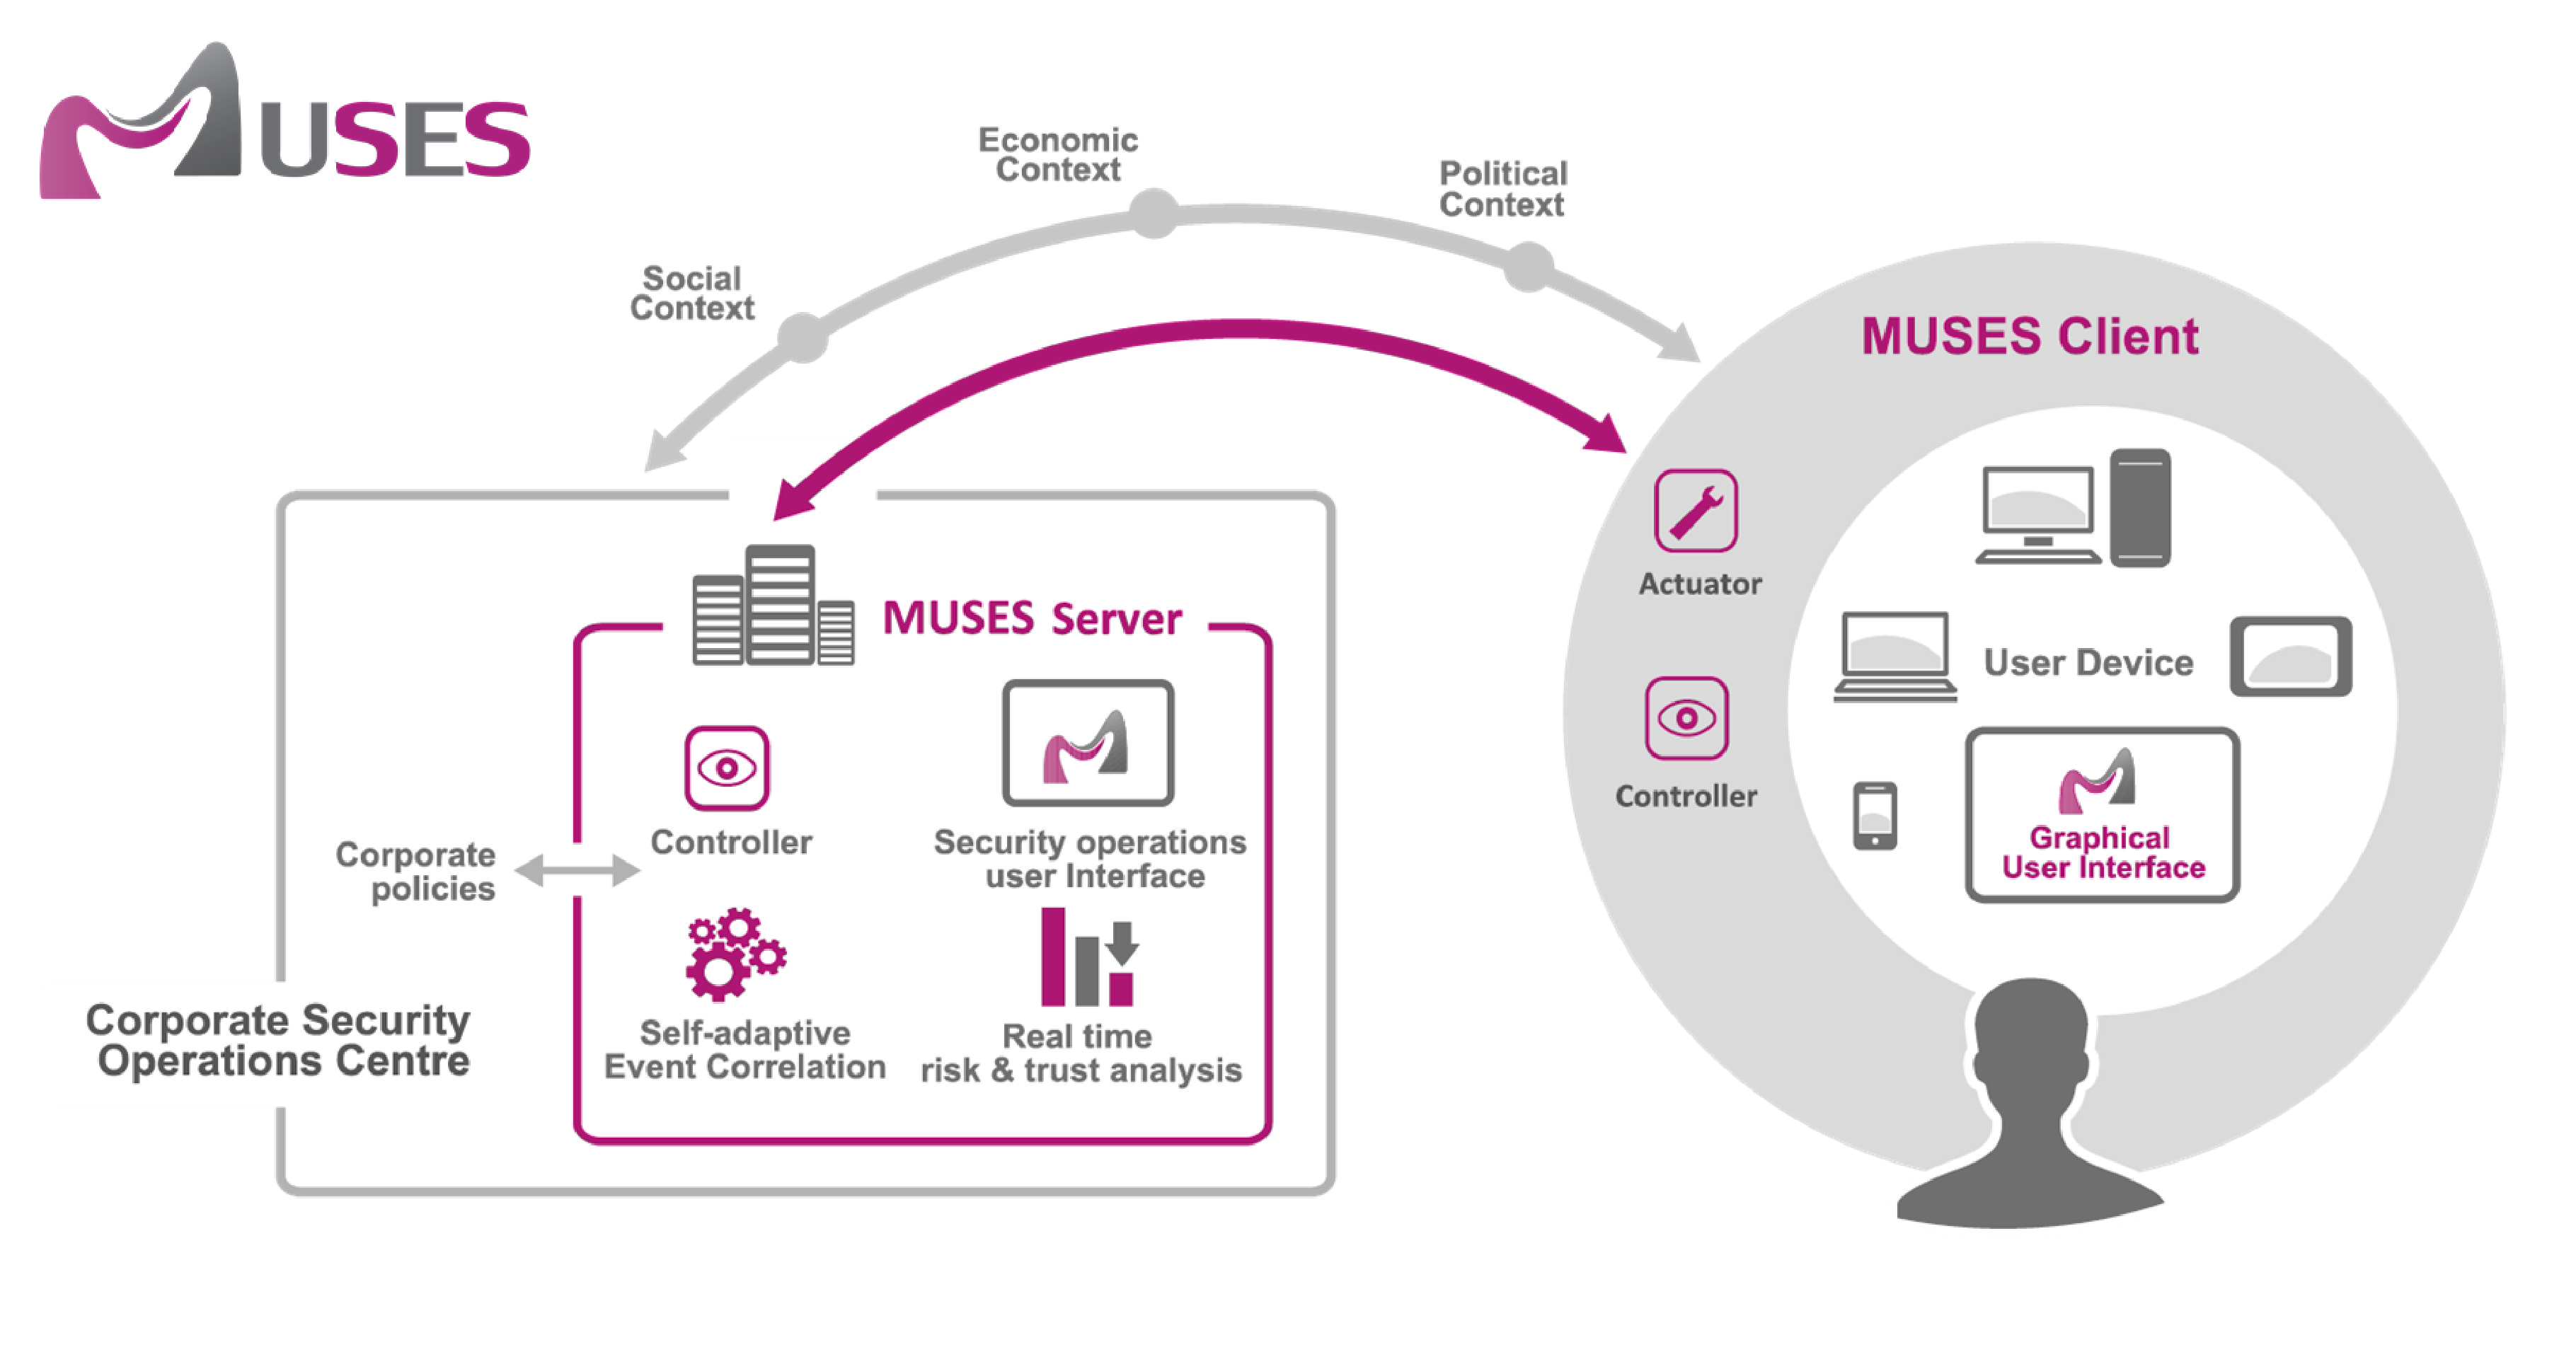
\includegraphics[scale =0.17] {gfx/byodSotA/system_overview.eps}
\caption{MUSES system overview. Conceptual model designed by S2 Grupo.  \url{http://www.s2grupo.es/}}
\label{fig:system_overview}
\end{SCfigure}

As a summary, this application includes two modules: a \textit{controller} and an \textit{actuator}. The former consists of a number of implemented \textit{sensors} in the device, which monitor the environment and the users' behavior \footnote{Which has been introduced as the `context' of an event.}. Then, the user's actions, as well as device configuration, or connection properties, are translated into a sequence of events. These events, along with the stored patterns defining the user's conduct, are processed by the system in real-time by means of a Risk and Trust Analysis Engine (RT2AE) and an Event Correlation module. Then, a decision is taken in the corporate Security Operations Centre (SOC) side, considering the RT2AE output and the set of security rules adapted to that specific user and context. The corresponding feedback is communicated to the user through the \textit{actuator}, and then the user decides to comply or not with the policy. As mentioned before, MUSES depends on the MUSES Aware applications to be able to really stop the application if the risk is dangerously high. In case that MUSES cannot kill the application process, and if the user decides to continue performing a risky action, the user trust value will decrease and the CSO will be notified.

MUSES architecture is shown in Figure \ref{fig:architecture}. It is a \textit{client/server} approach in which the \textit{client} application can be installed in every user's mobile or portable device, independently of the platform. MUSES client is available up to date to be used in Android devices as well as in Windows mobile devices and PCs; the iOS client is under development. The same sensors are available in Android and Windows, but there is a strong limitation with monitoring iOS devices if they were not been \textit{jailbroken}. This means that if an iOS device has not been rooted, MUSES could not monitor every process in the device, and also it would have access only to some sensors. However, to be rooted is one of the situations that MUSES tries to avoid, which is why it depends on MUSES Aware apps. As far as the server is concerned, it has been developed using Java to be installed with an Apache Tomcat in the corporate server, independently of its OS. Both sides are connected through a secure channel using HTTPS over the Internet. Figure \ref{fig:architecture} only shows the high-level components in each part, along with the way the information flows in the system.

\begin{SCfigure}[tb]
\centering
 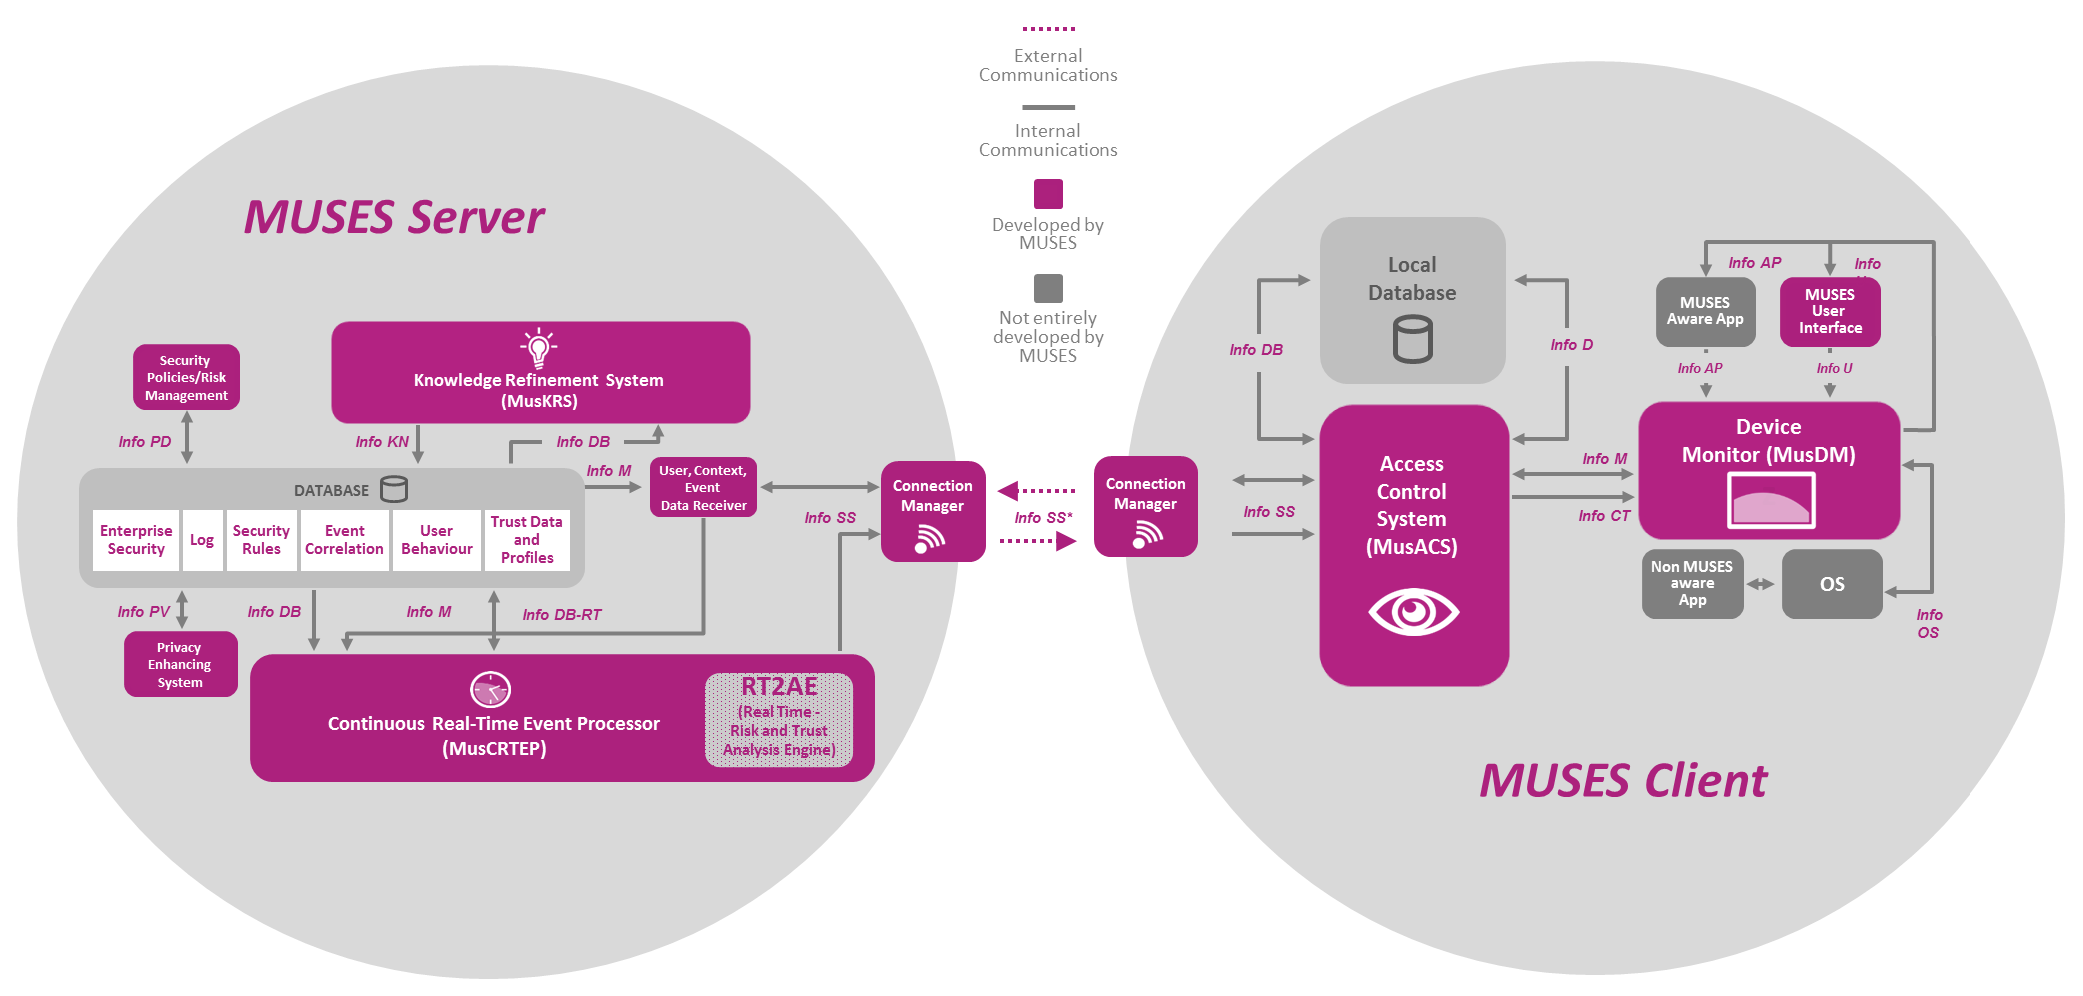
\includegraphics[scale =0.32] {gfx/byodSotA/architecture_modules.eps}
\caption{Design of the MUSES architecture (art by S2 Grupo).  \url{http://www.s2grupo.es/}}
\label{fig:architecture}
\end{SCfigure}

The use of a server is mainly based on the need of a powerful machine, able to work with massive amounts of data (\textit{Big Data}) \cite{BigData_11}, since the algorithms to apply to them require high computational costs \cite{Shirkhorshidi14Review}.
Moreover, part of the high computational cost methods to apply needs to be derived to this high-performance server, as the mobile devices do not count with enough computational power. These methods include DM \cite{DataMining_Lee01} and ML \cite{MachineLearning_Bishop06} techniques, which have been proved to be computationally expensive \cite{Cios07DataMining}. This server is also devoted to centralize the data gathering from all the devices in the company, composing a big database to which the commented techniques can be applied.

The system considers two working modes for every device: online and offline. In the \textit{online} mode the device can connect with the MUSES server, so that it can request the server to make a decision. On the other hand, in \textit{offline} mode the server cannot be reached by the device because there is not an available connection between them, so all the decisions are made locally.
This is done using an up-to-date copy on the Decision Table inside the Local database, which contains decisions for any type of detected event, along with the default actions to be performed if no rule is met. In this mode, the gathered information by the sensors in the device is stored for later submission to the server side when a connection is available, in order to be processed in the knowledge refinement process.
Moreover, when switching from offline to online mode, the device receives an updated copy of the Decision Rules, the so-called Device Policies, as a kind of antivirus database, in order to work again perfectly in offline mode if the connection is lost.

The MUSES system also performs an authentication process when the user logs in. The MUSES server authenticates to the MUSES client by means of a self-signed certificate. The authentication of the users is based on Spring Security, which is a Java EE framework that provides authentication, authorization and other security features for enterprise applications. When the user connects to the MUSES server for the first time, the MUSES client asks the server for the certificate, which is sent and installed in the client local database if the user credentials are right. As the user credentials are also stored in the MUSES client local database, the user can also log in to MUSES, and it therefore can apply the Device Policies. With regard to internal data security, MUSES makes use of the advantages that the OSs themselves offer to developers. More concretely, the first prototype for Android includes functionalities provided by the Android Application Sandbox \cite{blasing2010android}. This means that other applications cannot access MUSES data, nor even other developers. The only way to do this is by rooting the device, which is a state that MUSES can detect, and therefore warn about its implications. With regard to the encryption of the rest of the device data, MUSES stands for having a security policy which advices about the installation of existing open source tools, instead of having an own implementation.

% ----------------------------------------------------------

\section{Client/Device architecture}
\label{subsec:client}

There are three main components in this side:
\begin{itemize}
 	 \item \textit{Local Database}: it is a local security-based storage, which includes the set of security rules to be applied locally (Device Policies), user authentication data, and a cache of gathered events and information. The latter is useful when the device is in offline mode, so these events can be later submitted to the server side, when the device returns to online mode. 
%It contains the so-called \textit{Decision Table}, a set of rules in which the antecedents are high-level events, and the consequents are the corresponding decisions/actions, namely `allow', `deny' or `request' (the decision must be made in the server side).
 	 \item \textit{Device Monitor (MusDM)}: module which contains the two main described modules, controller and actuator. When a user performs an action, an event is automatically created and either sent to the server (online) or locally stored (offline). In addition, there are several sensors implemented in the system which periodically scan different aspects of the device configuration and the environment. This way, the system acts equally over specific actions, as well as when it detects something from the sensors that is against the security policies.
 	 \item \textit{Access Control System (MusACS)}: module in charge of making the decisions considering the gathered data. These decisions can be made locally if possible, or can be requested to the server if there is no rule which matches with the occurred events. 

%The subcomponents are the \textit{Decision Maker}, which performs the decision process; the \textit{User, Context, Event Handler}, which processes the events and information to be used for making the decision or stored for further submission (depending on the mode and on the gathered data); and the \textit{Security Policy Receiver} that updates the set of decisions (or Device Policies) in the Decision Table with those received from the server side, after an update or decision process.
\end{itemize}

The client is an important part of the a-priori risk treatment, because it both monitors the whole context, and finally acts or warns the user in event of a security violation. 
% Antonio - yo pienso que en este sistema cualquier violación de seguridad que se detecte se hará por medio de las reglas de seguridad. Eso sería lo ideal, pero para ello el CSO debe definir un conjunto que asegure la seguridad del sistema en la mayoría de casos. Luego el KRS podrá proponer nuevas reglas a través de 'predicciones' (inferencias) o refinamiento, pero estas últimas se construirán como reglas optimizadas para tratar con incidentes de seguridad ya detectados. No se pueden crear de la nada reglas para tratar con nuevos incidentes (desconocidos).
But security violations are mainly identified by security rules, which is why MUSES needs at least an initial set of rules, defined by the CSO. Then, it makes use of DM and CI techniques to improve or optimize them, enhancing the coverage. 
That is to say, the more sensors are implemented, the more information related to event context can be extracted. Implementing a sensor means to include a programmed method which triggers MUSES to start `listening' to some parts of a device. Then, the initial security rules establish which situations might cause a security violation, and the sensors provide with information which helps the MUSES server to identify events that are alike to the ones that are already known as dangerous.
% Antonio - esto no lo veo correcto. El meter más sensores no implica que se vayan a mejorar en mayor medida las reglas. Sino que se pueden controlar más formas de actuación de los usuarios.
% Yo o escribría como algo separado, por ejemplo "A way to enforce the security in these devices is the inclusion of more sensors, which would be able to detect more potentially dangerous behaviours by the users (and thus, security violations)" 
For these reasons, MUSES implements the following sensors:
% Para Pedro -> El caso es que "sensors" es su nombre dentro del sistema. ¿Estaría mejor su pusiésemos "monitoring sensors"?
% Antonio - yo quitaría el 'for this reason'

\begin{description}
  \item[Connectivity sensor:] It gathers all information related to network communications, in addition to security properties like network encryption, or number of neighbours. This allows MUSES actuator to forbid the user for sending important emails, or opening key assets if, for instance, the network encryption is not secure enough. 
  \item[Device protection sensor:] Which scans device security settings, such as the time until the device screen turns off, if the device has the screen protected with a password, or if the device is rooted \cite{hildenbrand2014}. This security mechanism adds the possibility of detecting security violations even if the user is not doing a specific action.
  \item[Location sensor:] User location can be obtained using the device GPS. Although, this might be taken against the preservation of user privacy. This is why MUSES allows the definition of a number of `zones', and therefore it only checks if the user is inside them or not, acting in consequence.
  \item[Mail sensor:] If the user is writing an email, MUSES client sensor can also check the email attributes. Thus, it can detect if the event context is dangerous, according to security policies and the RT2AE, before the mail is sent.
  % (Paloma) Pedro, aquí he cambiado el "is going to send" a "is writing" en vez de "is sending" porque en realidad lo que queremos es que se le avise antes de mandarlo, no cuando lo está mandando o lo ha mandado. Se explica después. ¿Cómo lo veis?
  \item[File sensor:] The type of file, also called \textit{asset}, is also very important for the application of security rules. Thus, this sensor aims to detect if some files might need more strict security policies, also depending on the rest of sensors.
  \item[App sensor:] It is in charge of monitoring the information about the application from which the user is performing the action, but also looks for installed trusted antivirus, and encryption applications. Additionally, this sensor gathers information about the applications which the user tries to install or uninstall.
\end{description}

It is important to note that MUSES does not work as an antivirus itself, but has a sensor which checks if the device has already an antivirus, and raises a security violation alert if not. It might happen then that the user ignores this advice and the device becomes compromised. As it would be explained in the next section, the sensors are constantly sending their monitored values, and therefore patterns are created, stored, and processed on the server. In case the device gets infected with rootkit-type malware \cite{bickford2010rootkits}, a sudden change in the values of the sensors will mean a significant change in the patterns. Then, this change in the patterns will be noticed by the server, which will immediately warn the user, and decrease the device trust value.

The rest of the components shown in the figure are: the \textit{MUSES User Interface (UI)}, the application through which the user interacts with the system; and the \textit{Connection Manager}, which controls the communications between MUSES client and MUSES server. 
In addition, there are two types of applications considered in this system. On the one hand, the \textit{MUSES Aware App} is an application adapted to MUSES, so the system can directly interact with it. This application must be implemented using the MUSES API (Application Program Interface). It should be noted that MUSES is an application that is running in the background, and third party apps can communicate with MUSES and ask for a response. Then, the MUSES API is not a normal API for building the third party application, but a collection of methods to allow this communication\footnote{The MUSES API is defined in the project, so for every application desired to be MUSES Aware, it should be implemented using this.}.
The main advantage of having MUSES Aware applications, is because actuator is able to actually forbid the users for doing something, if it implies a big risk for the company.

On the other hand, the \textit{Non MUSES Aware Apps} are those which MUSES cannot directly interact with. Usually, they can be accessed through the OS. But the type of information to gather from them and also the type of actions to do over them strongly vary depending on the OS, which should not be modified according to  \cite{Gessner13userfriendly}.
As was already mentioned, when MUSES is not able to close the application, a pop-up feedback message is automatically shown to the user. This message informs about why the action is considered as risky and what the user can do to avoid it.

% ----------------------------------------------------------

\section{Server architecture}

As in the client, we describe the three main components:
\begin{itemize}
	 \item \textit{System Database}: it stores all the information that the system can manage, including authentication data, enterprise security policies, values of the assets, 
% Antonio - no sé qué expresión será más correcta, pero deberíamos poner siempre "assets' values" o "values of the assets". Yo me inclino por la segunda.
user-related information (trust, context), events data, and, of course, security rules to apply with regard to the security policies.

	 \item \textit{Continuous Real-Time Event Processor (MusCRTEP)}: this component is the core of the MUSES system with respect to the decision making process. It includes an \textit{Event Processor}, the module in charge of performing the event correlation process \cite{deliverable21, deliverable52}. This is done by a so-called `Event correlation engine', which is in charge of taking the user action events that are sent from the device client, and analyzing them to look for an existing security rule that could be applied to the situation. The engine discovers that by analyzing the context events which are sent with the user action event, so that a complete model of the risks can be built. The output of this module is an `access request' which is sent to the \textit{RT2AE}. It considers the information included in the access request, as well as other information such as trust data and profiles, values of the assets, 
% Antonio - "values of the assets"
user reputation, or opportunity, to perform a risk and trust analysis task \cite{RT2AE_SOTICS13}. Finally, the RT2AE extracts the set of potential rules to consider in the analyzed situation, and these rules are therefore transformed into decisions (or Device Policies) and submitted to those devices to which they apply.

	 \item \textit{Knowledge Refinement System (MusKRS)}: this module is in charge of analyzing the information stored in the system database by means of Data Mining techniques, identifying relevant data, such as important patterns, key features, or security incidents. These are later processed for tuning up the existing set of rules, or for inferring new ones. The MusKRS component, along with the MusCRTEP, are what represent the extension of the state of the art in security solutions for a BYOD environment. 

\end{itemize}

There are some other components, which add extra functionalities to the system, namely:

\begin{itemize}
  \item A \textit{Security Policies/Risk Management} tool, that lets the company CSO to define and manage Security Policies and Rules in a friendly way. It also lets the management of risk-related information, useful for the RT2AE process, such as the values of the assets.
% Antonio - "values of the assets"
  \item  The \textit{Privacy Enhancing System}, which is a module aimed to fit with the legal compliance of the system regarding the user's data anonymization and retaining of these data in the system. There are three important points with relation to this matter \cite{deliverable72}. First, the data that the user provides to the system, such as name, or email, is only used for authentication purposes, so they are checked when the user logs in the system, but they are not used for Data Mining tasks. Then, the location of the device is never sent and stored in the database, but as stated in the previous section, there are a number of defined `zones'. What is checked is that the user is inside one of those zones of interest. For instance, a company might want to know if the user is inside or outside a zone defined as `company premises'. And finally, the use in MUSES of what is called as `soft limit' and `hard limit' \cite{deliverable72}. These limits exist to ensure the users that their data will not be kept longer than necessary. The soft limit is defined by the components that use the data (Event Processor, RT2AE, and Knowledge Refinement System) for decision making or rule refinement, but do not need that data anymore. In addition, the hard limit is provided by the law, in case that the employee leaves the company, or if there is a national law specifying a maximum data retention period.
  \item \textit{User, Context, Event Data Receiver}, which is devoted to receive data from the device side, such as events, or user-related data, and to distribute them among the components, storing in the database, and requesting the Event Processor to start the correlation task. Finally, there is another \textit{Connection Manager} which controls the communications with the device side. %FERGU: no usar etc en artículos, mejor poner: (events, user-related LOQUESEA, among others)
% Cambiado
\end{itemize}


% ----------------------------------------------------------

\section{Self-Adaptation in MUSES: The Knowledge Refinement System}

The self-adaptation, to the user and context, of the set of Corporate Security Rules is one of the main features of the MUSES system.
To this end, the \textit{MusKRS} module is in charge of analyzing all the gathered events, context, and user-related data. Then it processes the data and adapts or refines the security rules. This refinement is meant as an improvement of the existing security rules, and its aim is to deal with new, possibly insecure, events. As a result, a set of optimizations and additions to the set of security rules are proposed to the CSO of the company.

This procedure is composed by two main steps: first, a DM \cite{DataMining_Lee01} + ML \cite{MachineLearning_Bishop06} process is performed in the \textit{Data Miner} sub-component; second, a refinement and inference process is done in the \textit{Knowledge Compiler} sub-component, using the data that was extracted in the first step, and by means of CI techniques.
The refinement or adaptation of the security rules can be made through techniques as simpler as generalization or specialization of rules, for instance, or by more complex CI methods such as Evolutionary Algorithms \cite{EAs_Back96}.

Another important fact is that MUSES functionalities are completed by a human controller, normally the CSO, who supervises the system activity by means of a graphic interface they can interact with. 
% Antonio - Si estamos hablando en tercera persona del singular se suele poner 'she' para referirnos a una persona de cualquier sexo, pero me gusta más poner 'he/she' para no discriminar. En todo caso intentaré poner 'they' en lugar de 'he/she', pero aquí, tal y como está redactado 'they' no queda bien por el verbo. 
% Antonio - No lo cambio porque no sé tu opinión, no es por dar trabajo extra.
% A ver, este fenómeno gramático se llama "singular they", y se considera más correcto utilizarlo que poner "he/she". No es que me lo haya inventado yo :\
% Antonio - Ok, entendido. Es que nunca lo habia visto.
Thus, adapted and inferred security rules are not directly added to the current set of rules, but they are proposed instead as draft rules to this human controller, in order to be accepted if they are interesting and useful. The system also uses the acceptance or rejection of new rules as `feedback`, learning from these decisions, and refining the rules according to this.

The following sections describe these processes: first, focusing on DM techniques to be used both automatically by the MusKRS, and by the mentioned graphic interface for showing useful information to the CSO; second, used CI techniques are explained, mainly focusing in Evolutionary Computation (EC) \cite{EAs_Back96} approaches. EC methods have demonstrated to have a good performance, and have been widely used in security-based environments for solving security issues, such as intrusion detection \cite{GA_intrusion-majeed}, design and evaluation of security protocols \cite{GP_intrusion-lu,GA_networksecurity-zarza}, or for the optimization of different aspects related with security: IT security costs \cite{EAs_securitycosts-kirta}, and cryptographic protocols \cite{GA_cryptographicprotocols-zarza2}, among others.

% ------------------------------------------------------------------
%
\subsection{Data Mining + Machine Learning}
\label{subsubsec:dm_ml}

This task is performed by the \textit{Data Miner} module. It  takes the `raw' data from the database and processes the information, in order to yield a set of relevant data for the Knowledge Compiler module and for the human controller. In the first case, this Data Miner component takes the set of data as a reference for refining or adapting the current set of security rules, to deal with anomalous situations, for instance.

The set of data is composed by the so-called patterns, which consist of an occurred event 
% Antonio - quedaba raro decir que estaba formado por 'un evento' como tal
and all the related information to that event. This means that the context in which the event was, is translated into a number of \textit{attributes} of the pattern. 
%This process is mainly non-supervised. 
% Antonio - Lo que es no supervisado es la clasificación, pero si se está explicando de otra forma ya no tiene sentido decirlo.
Moreover, a lot of attributes are extracted from the events, for obtaining the more information as possible. 
During the first trials, a mean of 201 events per day and user was observed. By considering just a medium size company, of 250 employees, that would make an average of 50300 events per day, of which a high number of features are extracted. Furthermore, if for instance 6 months are considered for the `hard limit' (see previous section), the amount of events to be processed would exponentially grow, until reaching the 9 million events. For even bigger companies, this all result in huge datasets, so that MUSES makes use of several Big Data processing methods \cite{BigData_11}, such as: 

\begin{itemize}

\item \textit{Pattern Mining} \cite{PatternMining_Han07}: 
From the whole set of patterns which form the built dataset, the most frequent, as well as the uncommon, are obtained. The idea is that infrequent patterns are potentially suspicious, and thus, could be of interest to be checked by the CSO, or to serve as a reference for the rule-refinement process.

\item \textit{Classification} \cite{classification_67}: 
This technique tries to train a model (classifier) able to associate every pattern in the dataset to a class, so that the model could be used for assigning a class for further incoming patterns with an unknown category.
Then, the model learns from events that, according to the ISPs, had been previously marked as `allowed' or `denied'. When a new event arrives to the server, if it has not an assigned decision, the classifier should provide one based on the similarity with previous, and already labeled, patterns.

\item \textit{Clustering} \cite{Clustering_Jain99}: 
The aim of this method is grouping the patterns considering some similarity criteria, in order to manage them as a set. This is used for providing data visualization mechanisms through a graphical interface. This would make easier to interpret data interaction and the distribution in clusters with respect to the different attributes, or features, of the patterns.

\item \textit{Feature Selection} \cite{FeatureSelection_Guyon03}: 
It consists of extracting the most important variables from the data. Feature selection techniques have been proven \cite{liu1998feature} to preserve the performance of the original feature set 
% Antonio - yo pondría 'quality' en lugar de 'performance'. Un dataset no tiene rendimiento, bajo mi punto de vista
in terms of classification accuracies, while significantly improve the processing time.

\item \textit{Data Analysis}: 
This provides the CSO with mechanisms to visualize interesting facts about the data, such as most frequent events, dangerous or suspicious users according to their behavior, most triggered rules, etc. All this information is shown to the CSO via the mentioned graphical interface, implemented in the server.

\end{itemize}

%\pagebreak

% ------------------------------------------------------------------
%
\subsection{Computational Intelligence: Evolutionary Computation Methods}
\label{subsec:ci}


MUSES uses different EC approaches, initially, two in the DM/ML part of the process, and three in the rule-refinement and adaptation phase. They are based on Genetic Programming (GP) \cite{GP_Koza92}, and Genetic Algorithms (GAs) \cite{GAs_Goldberg89}.

The Data Miner module adopts two evolutionary-based approaches. In the first place, a \textit{GP-based classification} method. This is useful for two main reasons: to deal with the data class imbalance \cite{imbalance_techniques_02}, which is very common in classification problems with real systems, gathering real data; and to better manage categorical data, since most of the features and information gathered from the events take these kind of values.
%, and being non-numeric does not allow to measure the distance between them.
% Antonio - claro que se puede medir la distancia entre valores no numéricos, lo que pasa es que normalmente, ésta no es representativa. Mejor omitir esto o poner de forma genérica que 'los valores categóricos dificultan el proceso de machine learning'.

Thus, this kind of classification method is able to manage unbalanced datasets, for instance, by considering a fitness function in which a cost is associated with the classifier accuracy at every iteration, having a penalty cost when the classifier makes a false negative. A false negative is an element from the minority class which is classified as belonging to the majority class \cite{cost_adjustment_07}.
With regard to the type of data, since GP algorithms can manage rule or tree based models, it works perfectly with any categorical feature, yielding a good classifier as it has been demonstrated in \cite{cost_adjustment_07}.

The second evolutionary approach taken in the Data Miner is the Feature Selection process that was mentioned in the previous section. This process is conducted using a GA as a meta-algorithm to test all the possible combinations of pattern features in the classification. Thus, the GA algorithm can optimize the group of features to be considered in the classification task, improving both the computational time of this task and also the obtained accuracy of the method \cite{liu1998feature}.

On the other hand, the refinement or adaptation of the security rules is performed by the \textit{Knowledge Compiler} module, and it uses three EC methods. These methods can be used for inference and optimization, and they use different data as part of the process, such as:
% [Pedro] maybe we should specify how the following data is used in each one of the 3 EC methods...

\begin{itemize}

\item The information extracted from the Data Miner sub-component, mainly concerning the anomalous, unclassified or misclassified patterns. These are those patterns which did not match with any of the existing classes, as they are quite different from the patterns belonging to those classes. This way, they cannot be included in any of the classes and thus they should be taken into account for a potential inference or update in the set of security rules, in order to `cover' them.

\item User-related information, and context information in general, corresponding to those anomalous or unlabeled events. Thus, the user's location zone, role, or device settings, for instance, can be considered in order to select the applicable set of rules for those conditions.

\item Risk information extracted from the user profile, e.g. ``Did the user received a lot of `denies' or `allows' before?'', in other words, ``Is the user trustworthy?''. In case the user is not, meaning that the user trust value is low, more restrictive rules can be created, otherwise the corresponding rules could be `softer' for that user.

\item The information about the user behavior with respect to system messages, whether the users acts in consequence or against MUSES advice, as well as user feedback. The user feedback has been measured in the MUSES trials by making interviews with the people who have used MUSES, but it can also be measured by pop-up messages, such as ``has this information been useful?''. 
% Antonio - quito el guión porque un revisor dice que se usan demasiados y que hacen el texto menos fluído y legible.
% Paloma -  "forward slash" no significa guión. Un forward slash es un / que sí había muchos en el texto.
% Antonio- Ok. En todo caso lo dejaría sin el '-type', pero como veas. Si lo quieres poner como estaba, el ', such as' lo añadí yo y lo mismo no queda bien así. 
% Ok pues con el such as.
All this information contributes to the inference of new rules or in adaptation, in order to deal with, for instance, users that repeatedly ignored warning messages.
Moreover, important log information with regard to the parameters used or the decisions made in the different modules can be used for further tests of new inferred rules, as it is explained below.

\end{itemize}

As the rule refinement process is considered of the same importance as inferring new ones, the following three approaches have been implemented:
% [Pedro] I'd change this to: "As the rule refinement process is considered of the same importance as inferring new ones, the following three approaches have been implemented:"
% or even to:
% "Due to the importance of the refinement process (it is considered of the same importance as inferring new ones) the following three approaches have been implemented:"

\begin{itemize}

\item A \textit{GP rule inference} method, which generates new rules in order to `cover' those situations that have been not contemplated in the current set of rules. Thus, a new rule would be created for dealing with the patterns to which the classifier could not assign a class.
The generation of new rules is done by considering the so-called \textit{dictionary}, i.e. a set of terms corresponding to all the possible context situations and user actions in the system, which are the antecedents and consequents \footnote{The antecedents are the conditions of a rule that have to be met to apply the consequents.} of the security rules to be inferred.
The evaluation of these rules is done by considering the information that has been described. Thus, it is possible to `simulate' the whole system behavior when the new rule is included. Therefore, the system gets a value of its performance in terms of, for instance, how many of the events that were not classified or misclassified, are covered now. As was also mentioned, the user or device trust values influence the creation of the rules.
Finally, the inferred rules are proposed to the CSO as ``new, but not yet refined'', along with their evaluated performance.

\item A \textit{GP rule refinement} approach, which optimizes the current set of rules, adjusting the values in the conditions. The set of rules that could be refined is composed by the new rules from the GP-based inference, but also by the original set of rules which was already completed by the Data Miner. Thus, some superfluous parts of the rules and even complete rules could be removed or improved, obtaining for instance specializations or generalizations of existing rules which could lead to a better performance. % [Pedro] change "could mean a better" to "could lead to a better"
The evaluation of the whole set of security rules is done by considering the number of unlabelled patterns that are `covered' after the adjustments. Again, the rules at the end of this step are presented to the CSO as ``refined''. The CSO is the one who decides, according to the performance simulation results, if an inferred rule, or the refined one, is the rule which is finally included in the system.

\item A \textit{GA optimization} algorithm for adapting the values of the assets. %FERGU: "values of the assets" mejor? Los valores no son "poseidos" por los assets, no? xD (tampoco tengo mucha idea del genitivo sajón, ojo)
% Toda la razón :D Se ma colao, shame on me!
These are numerical representations of the importance of the corporate assets, and are considered in the Real-Time Risk and Trust Analysis process, in order to assign a risk value to every potential decision that can be made by the system.
By evaluating the partial solutions proposed by the GA, this approach provides the CSO, who is in charge of assigning and adjusting these values over time, with information about the most dangerous situations for certain assets. In this process, then, the context information that is gathered by the system is very important. %FERGU: pondría el "in this process" al principio de la frase. % Ok, cambiado
The adaptation or adjustment concerns the change in the value that an asset has due to a loss of importance, for instance, for being an out-to-date document.

\end{itemize}

% [Pedro] it is not clear for me whether those 3 methods can be used (are used) independiently or one after the other(s).

As a summary, the Knowledge Compiler module uses two EC-based processes for inferring and refining rules, plus another one for adjusting values of the assets.
% Antonio - "values of the assets"
 Both the inferred rules and the refined rules are presented to the CSO, who includes them or not in the system, and this acceptance or rejection acts itself as a feedback for future rule inference.


% ---------------------------------------------------

% Antonio - pongo esto en una sección nueva para que destaque más. Es muy importante para los revisores. Por favor Paloma, revisa si lo que he puesto es correcto (número de usuarios y demás).
\section{Trials and tests of MUSES}
\label{subsec:trials}

A MUSES first prototype, implemented for Android devices, has been recently tested. These trials have been conducted in an actual Spanish company, with 50 employees using the system on their own devices.
% He quitado "(a partner in the European Project where the system is being developed)" porque creo que es irrelevante, y si no se puede redactar de manera que esté fuera de los paréntesis, no debería estar.
The trials were divided in two phases: \textit{silent} and \textit{verbose}, 1 month duration each. During the \textit{silent} phase, MUSES was able to gather data, but without warning the users when a security incident was happening. A total of 23358 security violations were detected. In the \textit{verbose} stage, MUSES started to show warning pop-ups to the users, every time a security incident happened. 

As results, not only the number of security violations were reduced by half in the first two weeks (10977), but the number went on decreasing until it was 0 even before the trials period finished. Thus, we can assume that MUSES is an effective tool, even though it has the limitation of needing an initial set of defined security rules to start working (this will be better explained in Section \ref{sec:comparison}). For this, MUSES also includes a set of guidelines for the companies to build adequate security policies. For instance, the set of initially defined rules used for the trials included a blacklist of forbidden applications, a whitelist of allowed ones, and requirement of antivirus, among others.

With respect to the computational costs, in this first prototype it takes less than 0.5 seconds in the client side, if there is already a decision in the local table for the happened event. Otherwise, i.e. if there is need to ask the server to make a decision (by means of Event Correlation + Risk and Trust Analysis), the time grows up to 2.5 seconds in the worst case.